% Chapter Template

\chapter{Ensayos y resultados} % Main chapter title

\label{Chapter4} 

En este capítulo se describe el proceso de verificaciones y validaciones que se realizó a fin de comprobar el correcto funcionamiento del sistema y el alcance de los objetivos del trabajo.

%----------------------------------------------------------------------------------------
%	SECTION 1
%----------------------------------------------------------------------------------------

\section{Verificaciones técnicas}



\subsection{Verificación del set-up de dependencias Ethereum}

Como se mencionó anteriormente para poder interactuar con la red Ethereum se necesita disponer de saldo en ETH en un wallet y para esto se utilizaron Faucets de Google. En la siguiente figura \ref{fig:google_faucets2} se puede apreciar la verificación de la obtención de tokens.

\begin{center}
   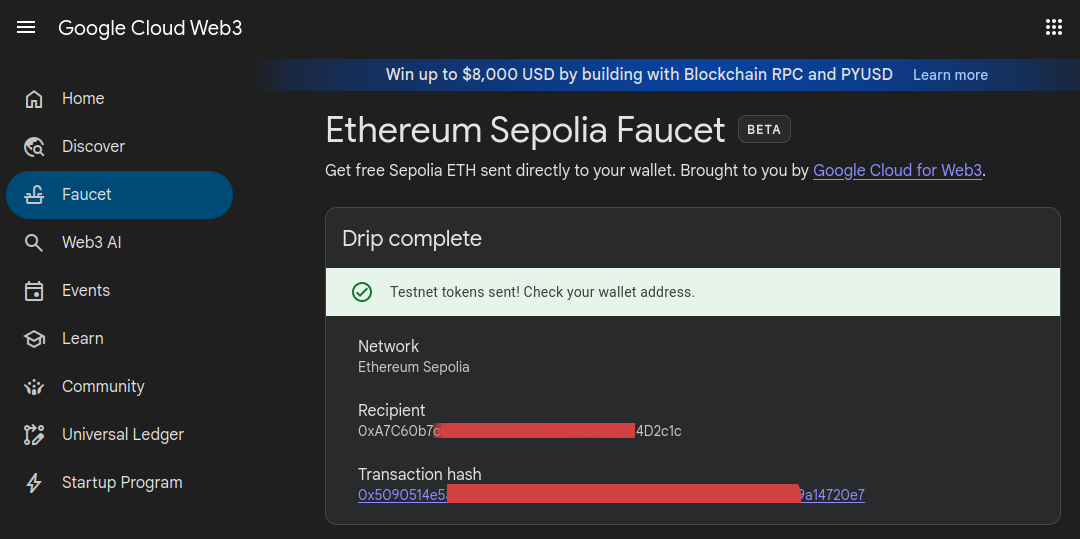
\includegraphics[scale=0.35]{blockchain/google_faucets2}
   \captionof{figure}{Obtención de créditos mediante Google Web3.}
   \label{fig:google_faucets2}
\end{center}

En la figura \ref{fig:metamask_balance} se puede verificar la acreditación de los fondos obtenidos en la billetera Sepolia utilizada para las pruebas. 

\begin{center}
   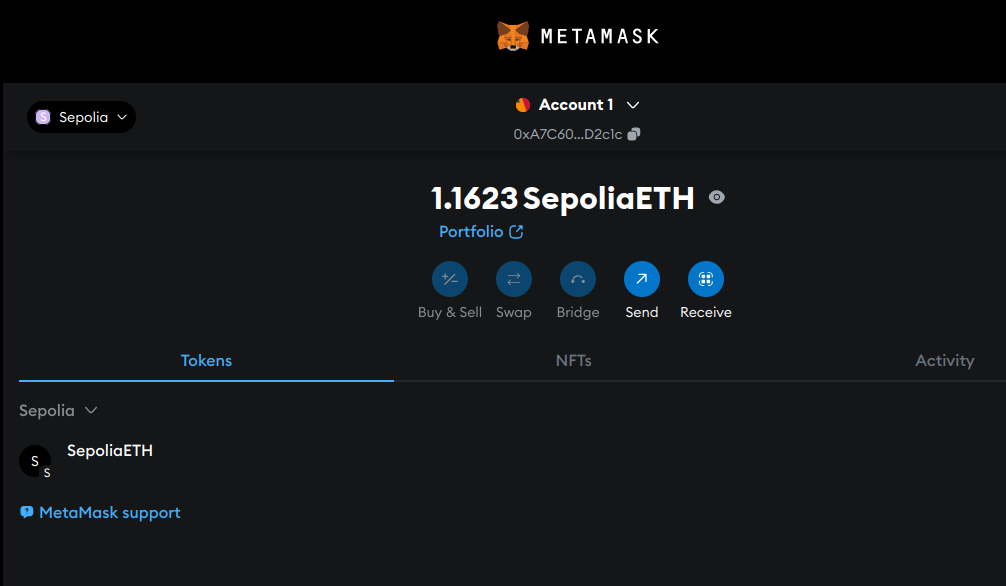
\includegraphics[scale=0.35]{blockchain/metamask_balance}
   \captionof{figure}{Saldo en Metamask.}
   \label{fig:metamask_balance}
\end{center}

Posteriormente se pudo verificar desde Etherscan las transacciones realizadas en la transferencia de los fondos via faucets \ref{fig:sepolia_funding2}.

\begin{center}
   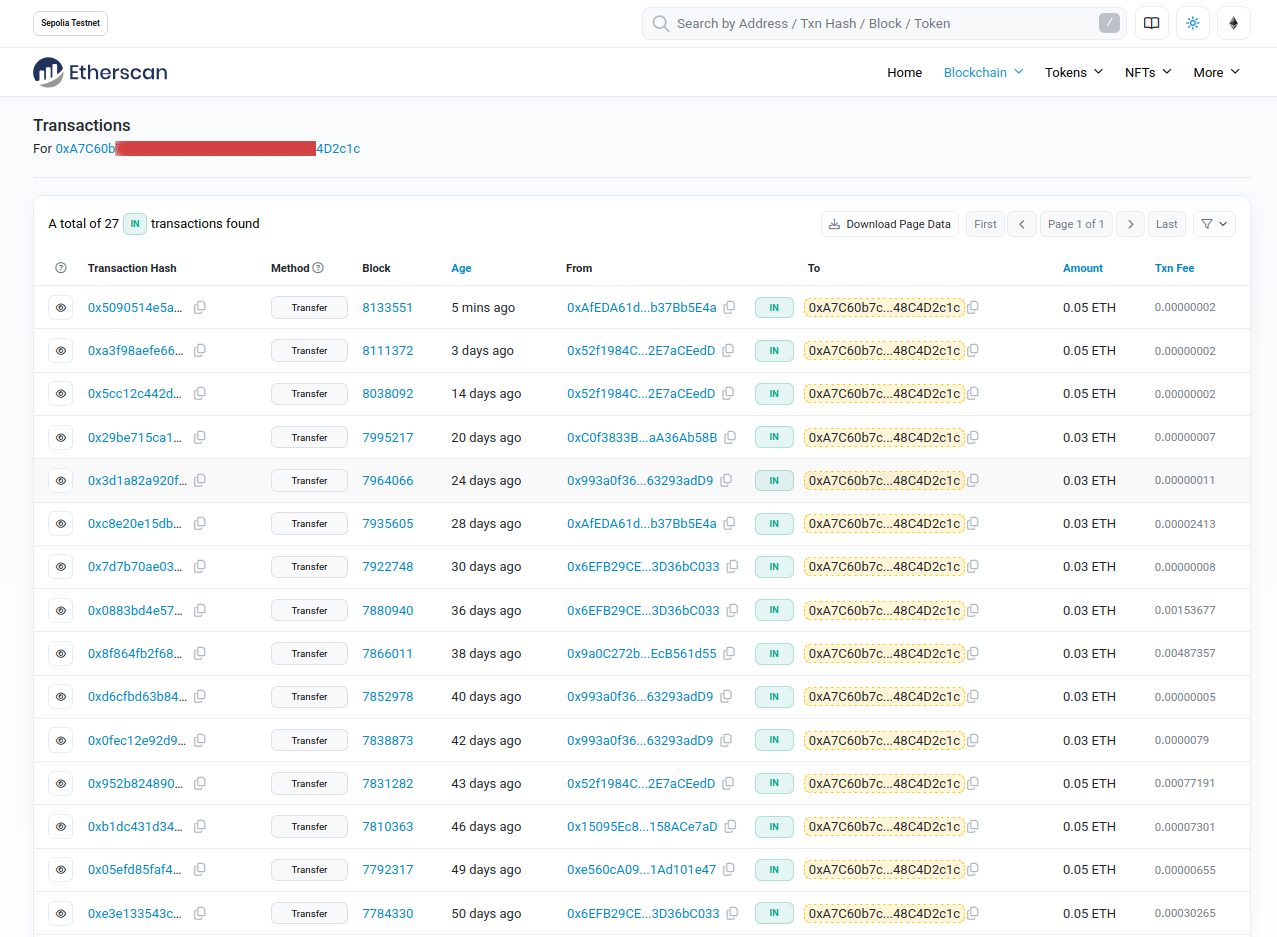
\includegraphics[scale=0.3]{blockchain/sepolia_funding2}
   \captionof{figure}{Transacciones de generación de fondos de prueba.}
   \label{fig:sepolia_funding2}
\end{center}

Como se mencionó anteriormente, el acceso a la red Ethereum se realizó a través del servicio Alchemy. En la siguiente figura \ref{fig:alchemy1} se puede apreciar la verificación de su set-up para poder ser invocado por la dApp. 


\begin{center}
   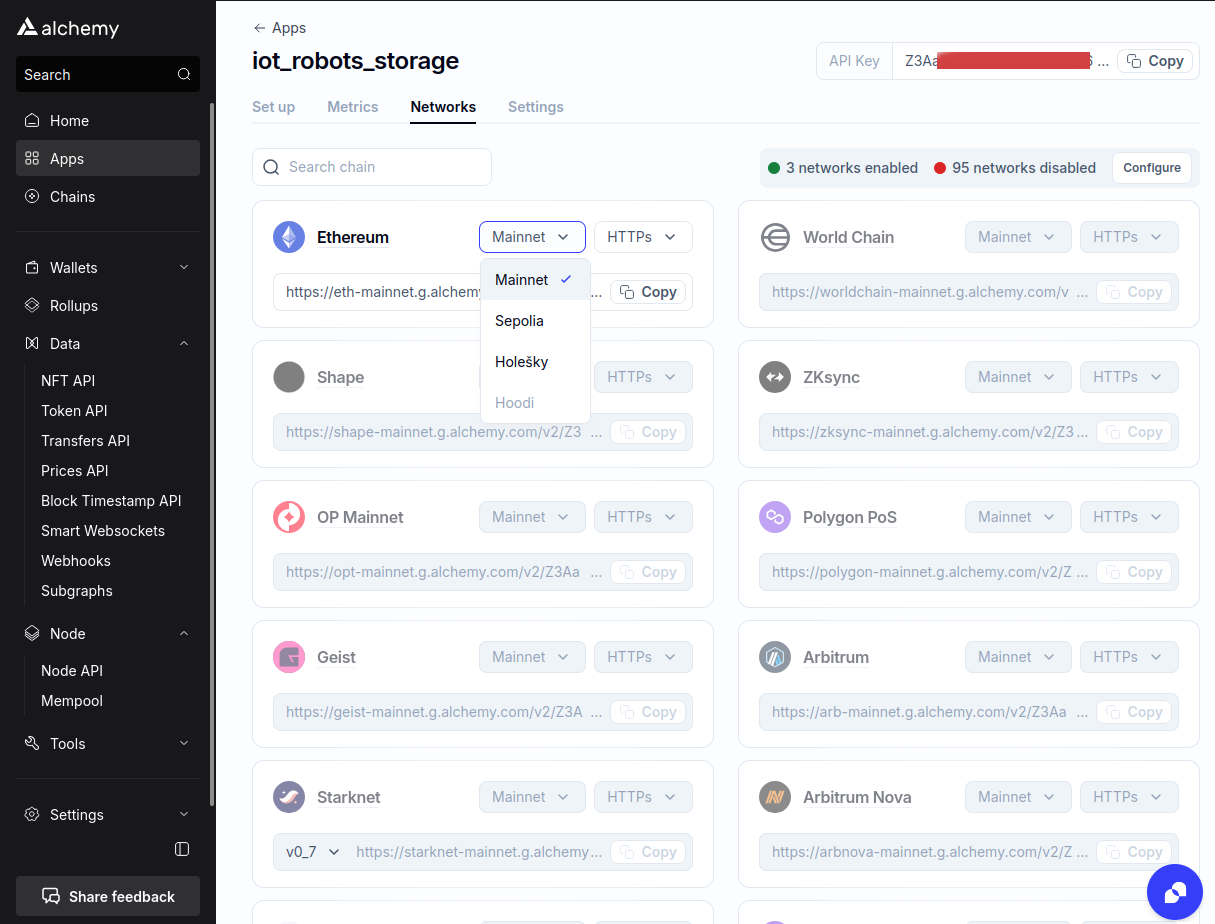
\includegraphics[scale=0.3]{blockchain/alchemy1}
   \captionof{figure}{Frontend the Alchemy.}
   \label{fig:alchemy1}
\end{center}




\subsection{Verificación del despliegue de los Smart Contracts}

Tras ejecutar el proceso de despliegue se pudo verificar la salida por consola con la confirmación del resultado exitoso. Como se puede apreciar en la figura \ref{fig:sm_deployment} se observa la dirección de los Smart Contracts, la cuenta, balance y gas utilizado.


\begin{center}
   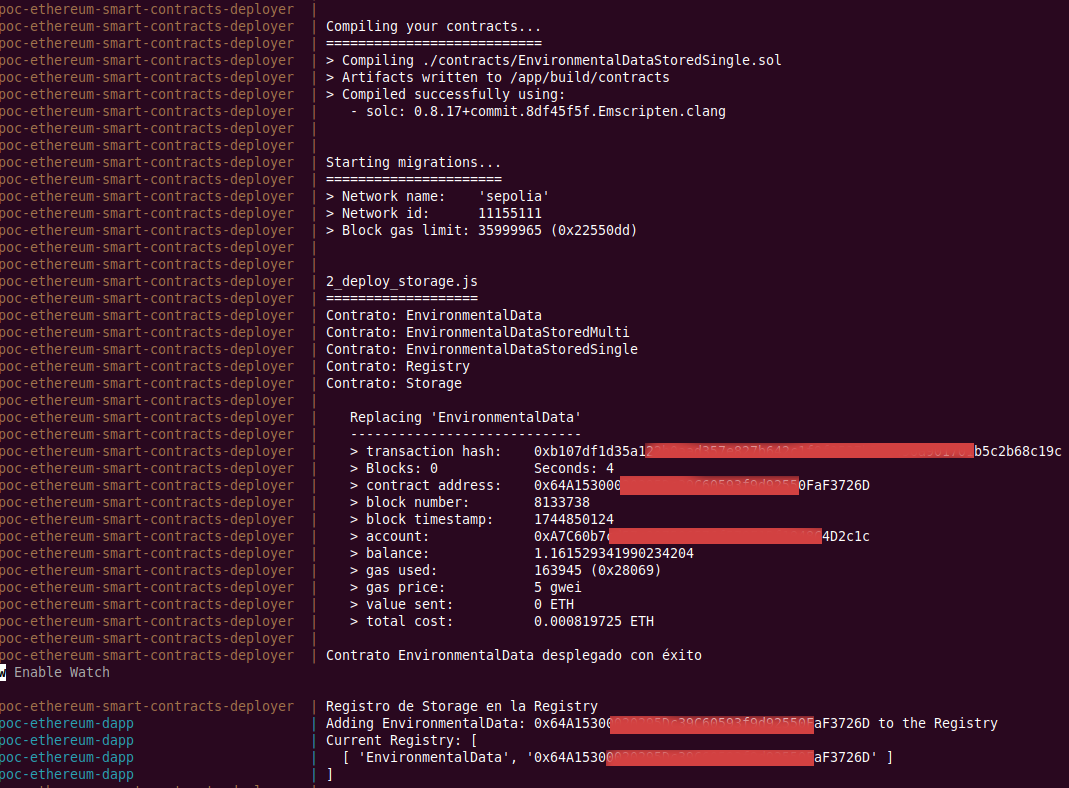
\includegraphics[scale=0.35]{blockchain/sm_deployment}
   \captionof{figure}{Salida por pantalla durante el proceso de despliegue de los componentes blockchain.}
   \label{fig:sm_deployment}
\end{center}

Posteriormente, desde Etherscan se pueden apreciar las transacciones de cada despliegue en la red, por ejemplo en este caso Sepolia, con los detalles de cada una de las operaciones.

\begin{center}
   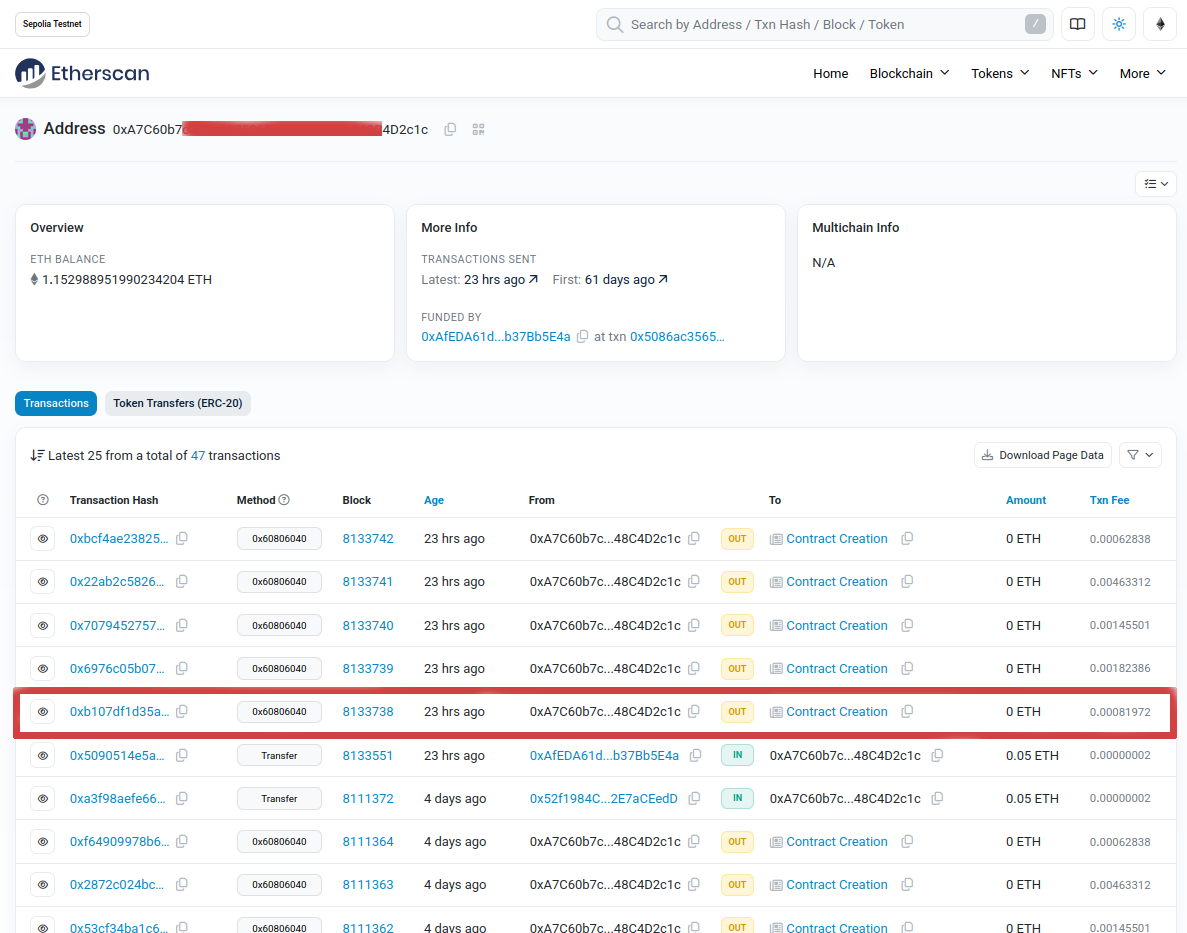
\includegraphics[scale=0.35]{blockchain/sm_deployment_etherscan1}
   \captionof{figure}{Transacciones de despliegue en Sepolia.}
   \label{fig:sm_deployment_etherscan1}
\end{center}

\begin{center}
   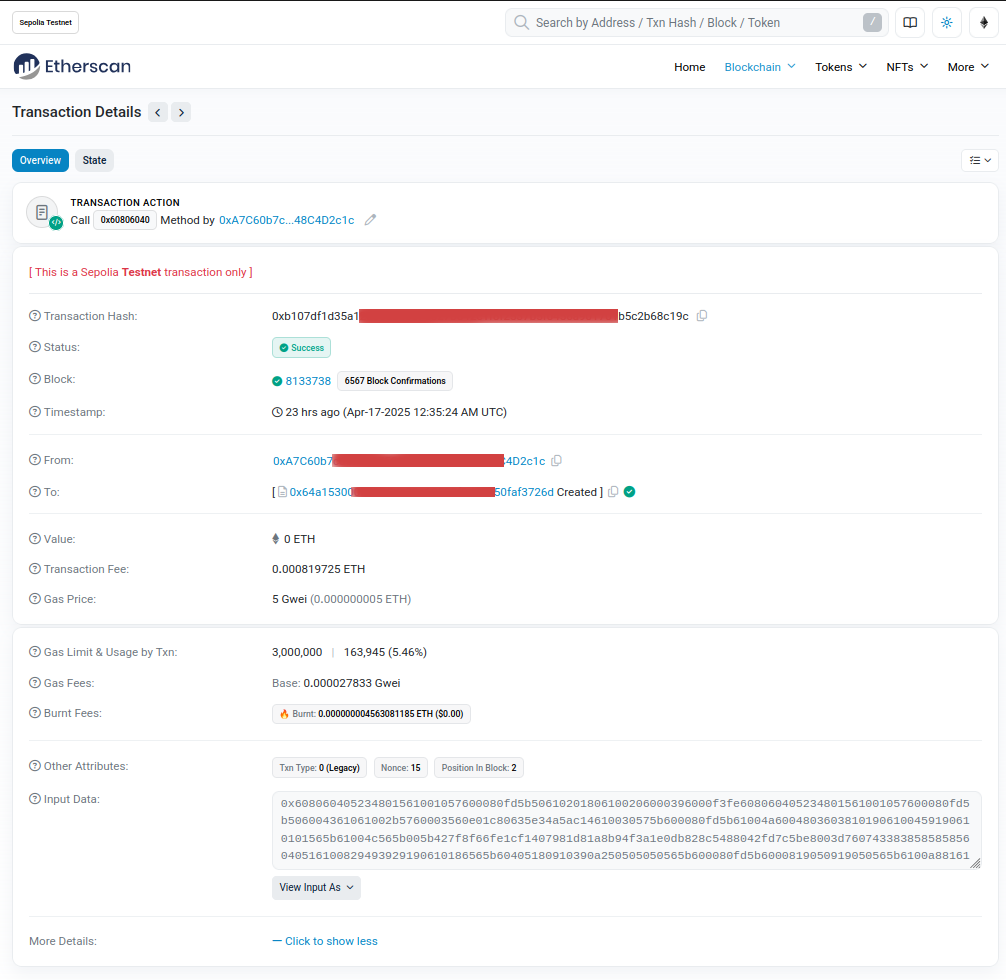
\includegraphics[scale=0.35]{blockchain/sm_deployment_etherscan2}
   \captionof{figure}{Detalles del contrato desplegado en Sepolia.}
   \label{fig:sm_deployment_etherscan2}
\end{center}



\subsection{Verificación del despliegue de la dApp}

Al realizar el despliegue por la consola web de AWS se puede apreciar el resultado exitoso del proceso. Como se observa en la figura \ref{fig:deployment_dapp}, tras el despliegue se puede obtener la URL desde la que se puede acceder a la dapp.

\begin{center}
   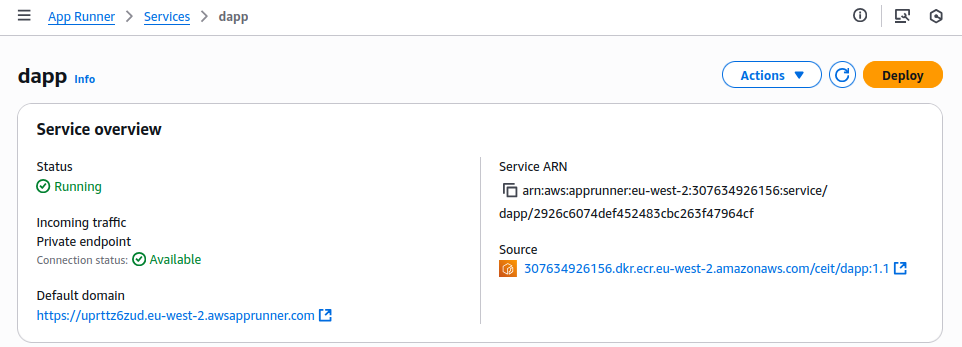
\includegraphics[scale=0.4]{AWS/deployment_dapp}
   \captionof{figure}{Despliegue de la dApp en App Runner.}
   \label{fig:deployment_dapp}
\end{center}

Como se puede apreciar en la siguiente figura \ref{fig:deployment_dapp_log} los logs del despliegue indican que el proceso se realizó exitosamente y se puede apreciar el historial de últimos despliegues.

\begin{center}
   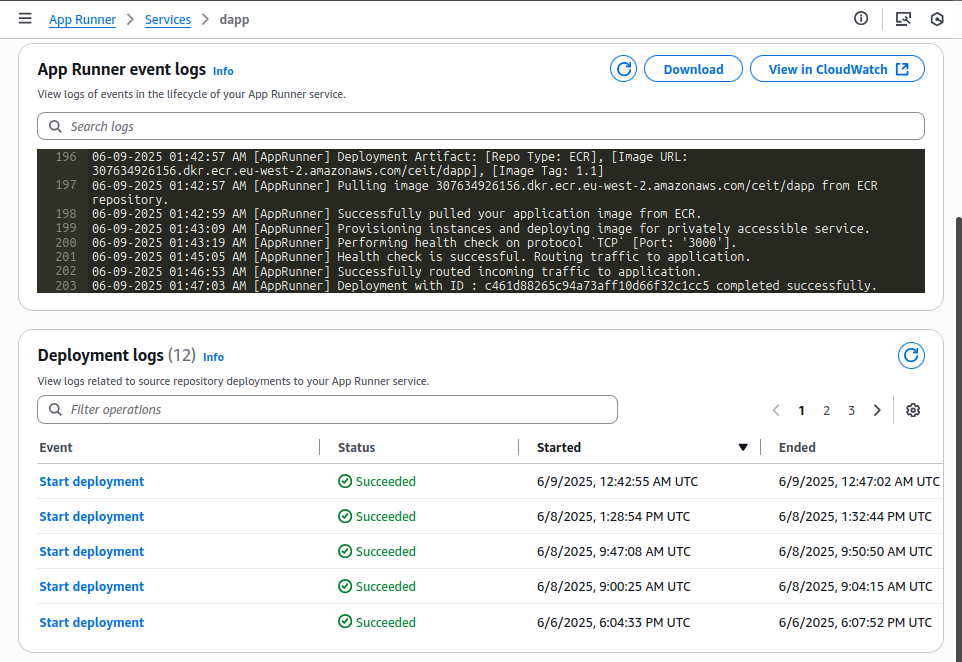
\includegraphics[scale=0.4]{AWS/deployment_dapp_log}
   \captionof{figure}{Despliegue de la dApp en App Runner.}
   \label{fig:deployment_dapp_log}
\end{center}

Una vez verificado el despliegue en la consola de AWS se puede apreciar en la figura \ref{fig:dapp_endpoints} la verificación del funcionamiento de la dApp accediendo a su API Restful publicada por Swagger.


\begin{center}
   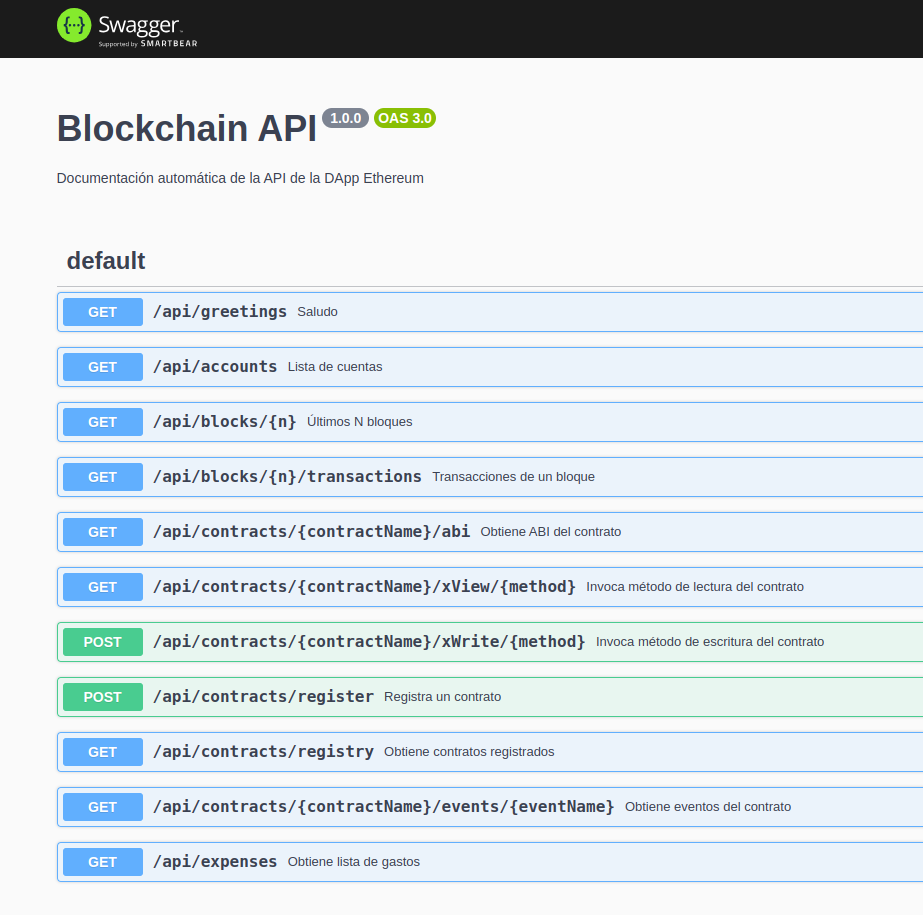
\includegraphics[scale=0.4]{blockchain/dapp_endpoints}
   \captionof{figure}{Endpoints expuestos por la dApp.}
   \label{fig:dapp_endpoints}
\end{center}


\subsection{Verificación de ingesta de datos en tiempo real MQTT}

Desde la herramienta AWS IoT Core se pudo verificar la recepción de mensajes MQTT desde el dispositivo ESP32 como se puede apreciar en la siguiente figura \ref{fig:aws_iot_core_mqtt_test_2}.

\begin{center}
   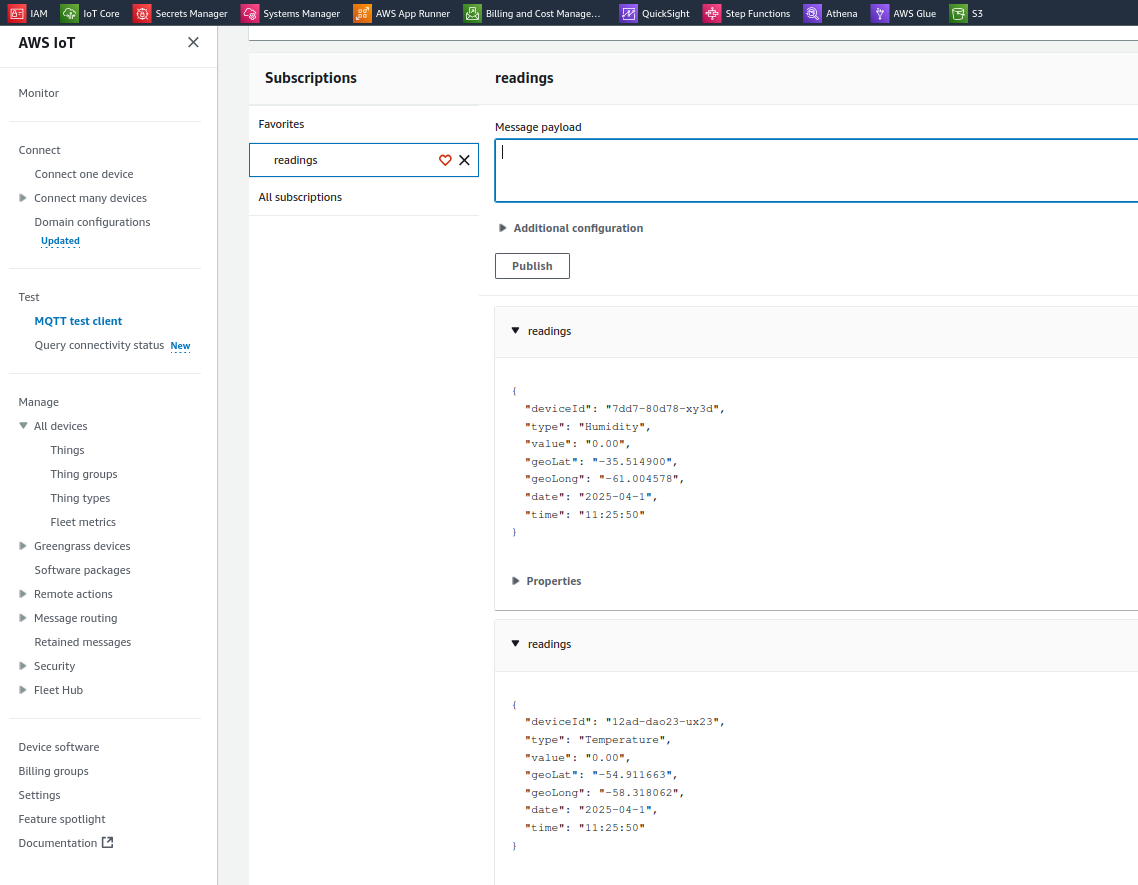
\includegraphics[scale=0.35]{AWS/aws_iot_core_mqtt_test_2}
   \captionof{figure}{Prueba de recepción de mensajes MQTT.}
   \label{fig:aws_iot_core_mqtt_test_2}
\end{center}


\subsection{Verificación del procesamiento de mensajes }

Una vez redireccionados desde AWS IoT Core por medio de AWS SNS, se pudo verificar el encolamiento de los mensajes en AWS SQS donde como se puede apreciar en la figura \ref{fig:events_sqs_2}, los mensajes se acumulan para ser procesados en la cola \textit{readings}.

\begin{center}
   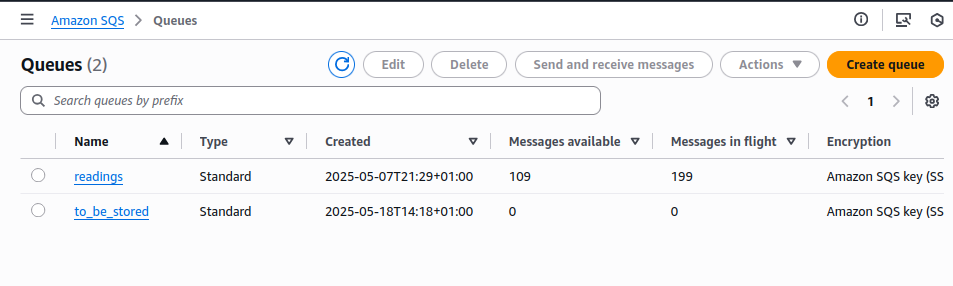
\includegraphics[scale=0.4]{AWS/events_sqs_2}
   \captionof{figure}{Configuración de redirección de mensajes MQTT.}
   \label{fig:events_sqs_2}
\end{center}

Como se aprecia en la siguiente figura \ref{fig:events_sqs_1}, también se pudo verificar la tasa de invocaciones de AWS SQS desde su herramienta de monitoreo.

\begin{center}
   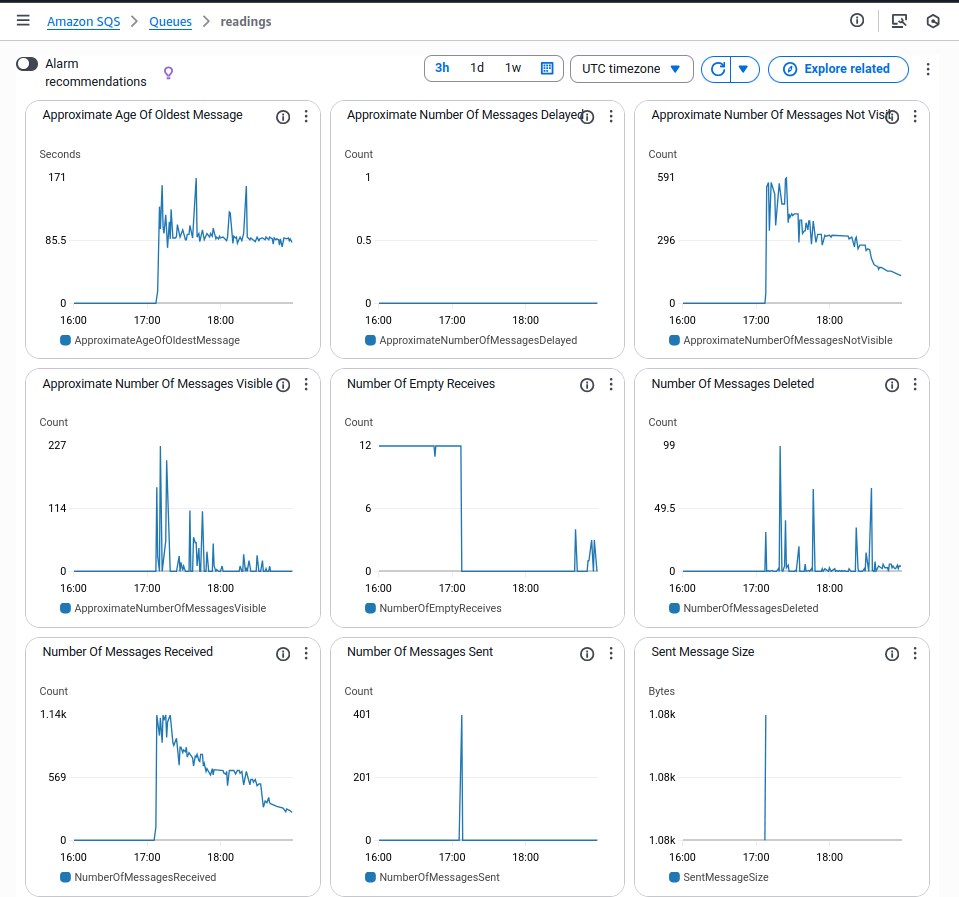
\includegraphics[scale=0.4]{AWS/events_sqs_1}
   \captionof{figure}{Configuración de redirección de mensajes MQTT.}
   \label{fig:events_sqs_1}
\end{center}


Como se mencionó anteriormente, desde la cola readings se dispara la ejecución de la función AWS Lambda que procesa los mensajes, invocando la dApp. Como se puede apreciar en la siguientes figuras \ref{fig:events_lambda1} y \ref{fig:events_lambda3}, se verificó el correcto funcionamiento del procesamiento de eventos.


\begin{center}
   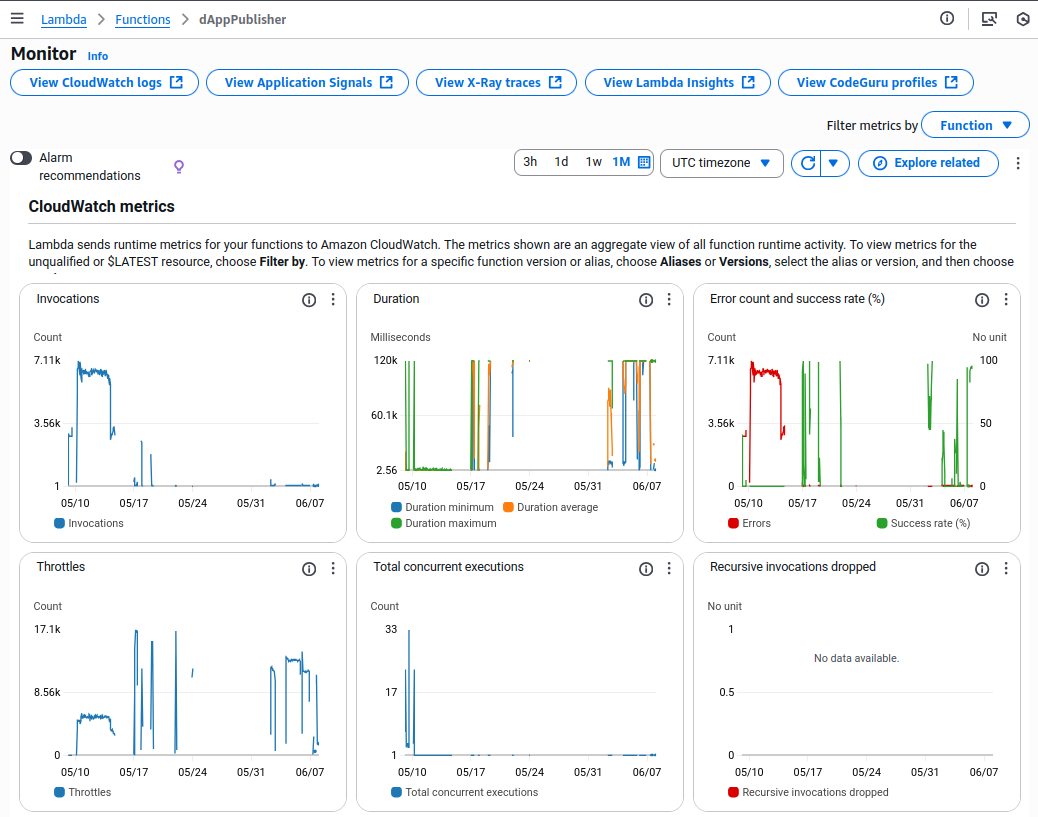
\includegraphics[scale=0.4]{AWS/events_lambda1}
   \captionof{figure}{Monitoreo de la función AWS Lambda de procesamiento de eventos.}
   \label{fig:events_lambda1}
\end{center}

\begin{center}
   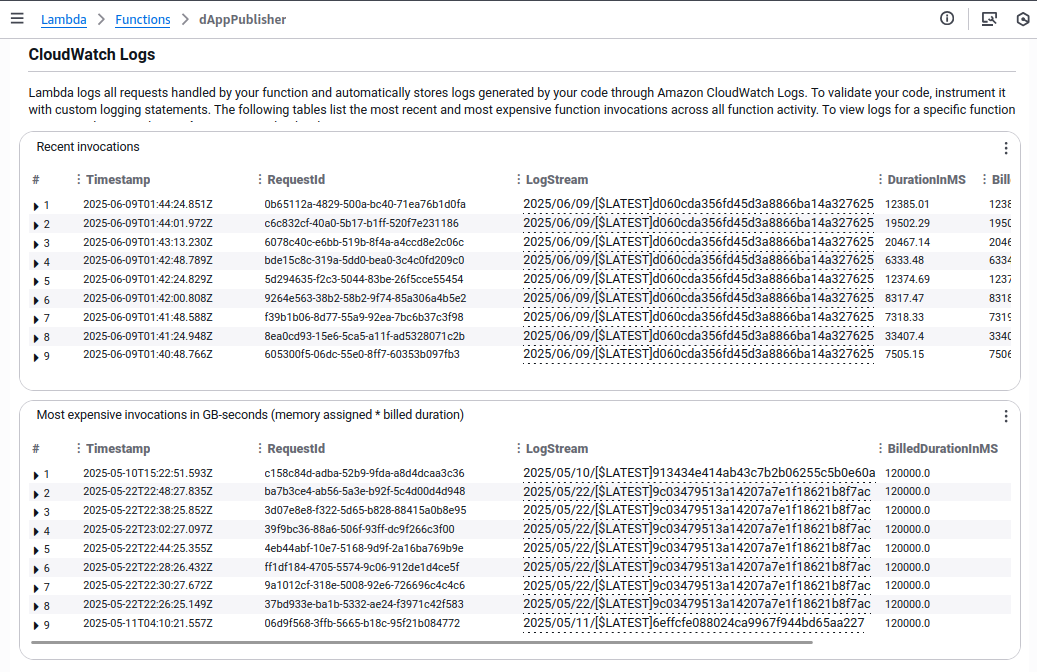
\includegraphics[scale=0.4]{AWS/events_lambda3}
   \captionof{figure}{Monitoreo de la función AWS Lambda de procesamiento de eventos.}
   \label{fig:events_lambda3}
\end{center}

\begin{center}
   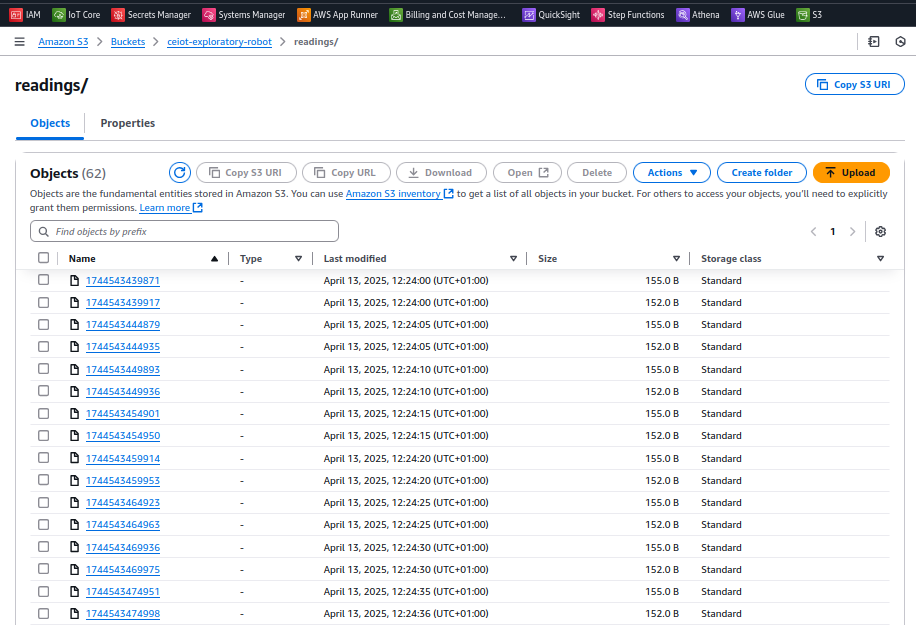
\includegraphics[scale=0.4]{AWS/aws_s3_bucket_data2}
   \captionof{figure}{Almacenamiento de mensajes JSON en AWS S3.}
   \label{fig:aws_s3_bucket_data2}
\end{center}



\subsection{Verificación de la invocación de la dApp y los Smart Contracts}

En la dApp, se pudo verificar el correcto funcionamiento del sistema en sus herramientas de monitoreo como se puede apreciar en las siguientes figuras \ref{fig:events_dapp} y \ref{fig:events_cloudwatch_dapp} las métricas de request HTTP y los logs de las transacciones Ethereum.


\begin{center}
   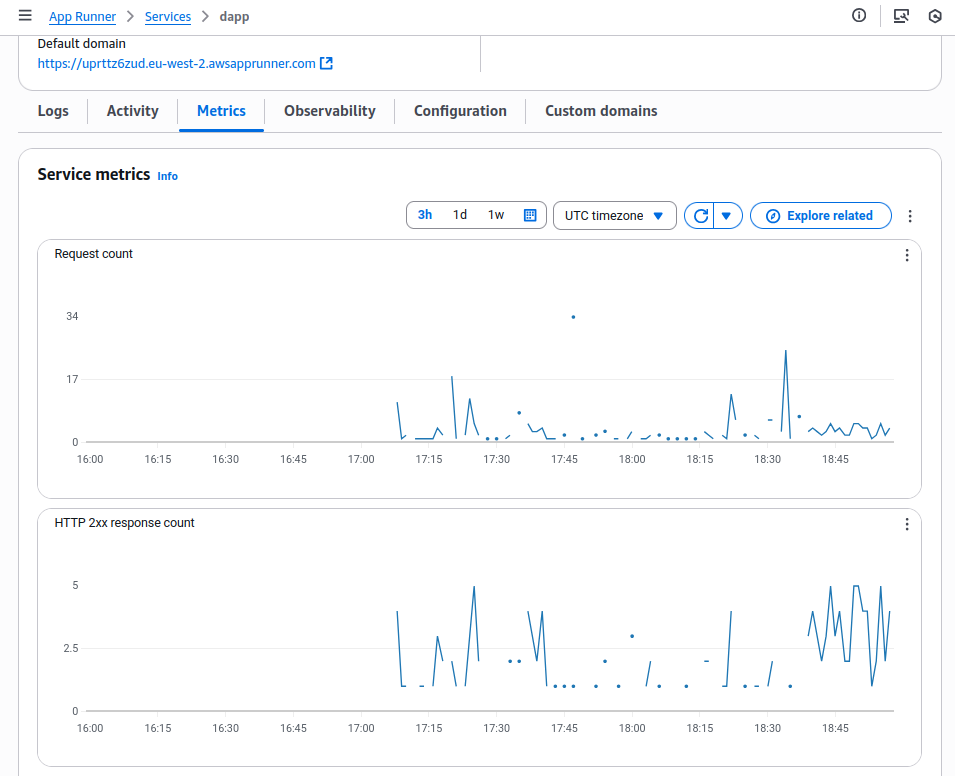
\includegraphics[scale=0.4]{AWS/events_dapp}
   \captionof{figure}{Almacenamiento de mensajes JSON en AWS S3.}
   \label{fig:events_dapp}
\end{center}

\begin{center}
   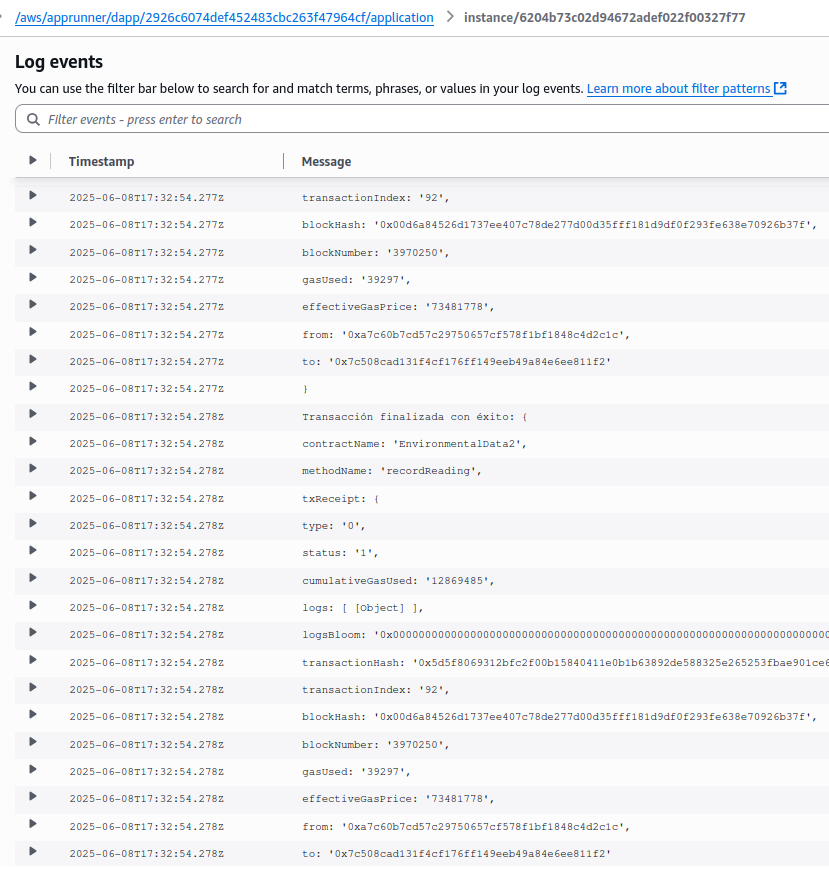
\includegraphics[scale=0.4]{AWS/events_cloudwatch_dapp}
   \captionof{figure}{Logs en Cloudwatch de las transacciones.}
   \label{fig:events_cloudwatch_dapp}
\end{center}


\subsection{Validación de los datos almacenados en Ethereum}


Por cada ejecución tambien se pudo verificar en Etherscan la creación de nuevas transacciones tras la ejecución de la dApp, como se puede apreciar en la figura \ref{fig:events_etherscan}.

\begin{center}
   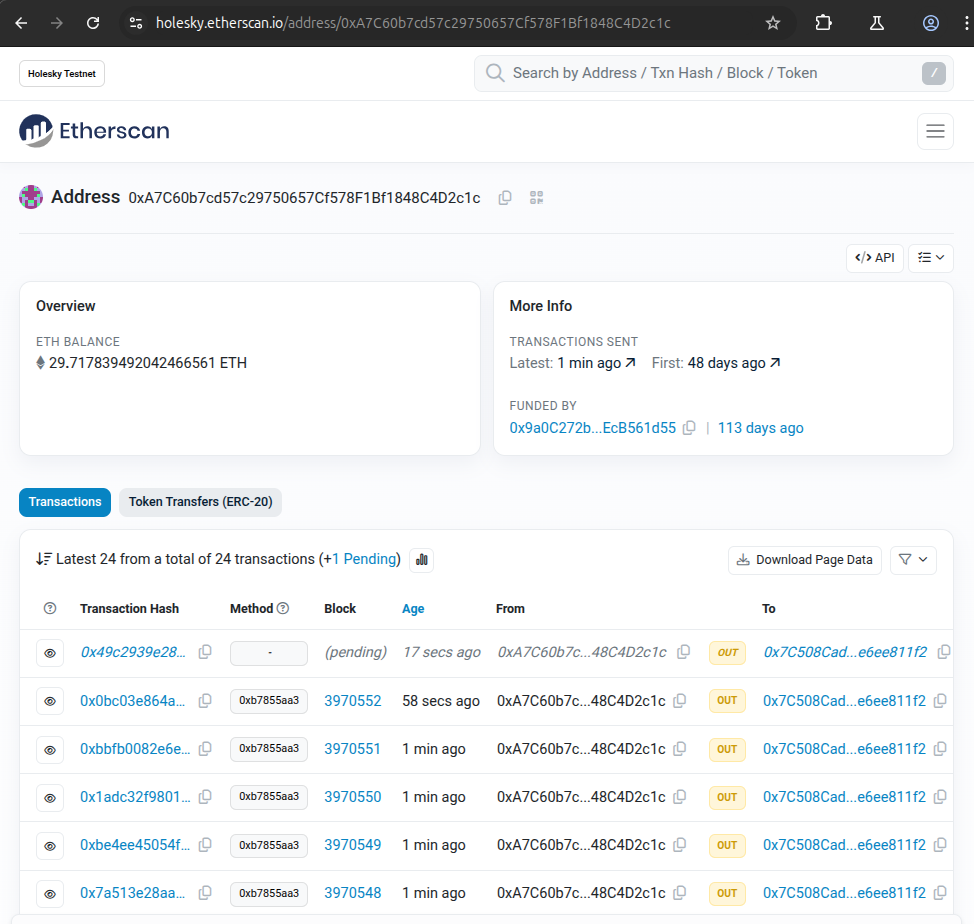
\includegraphics[scale=0.4]{AWS/events_etherscan}
   \captionof{figure}{Creación de nuevas transacciones en Etherscan.}
   \label{fig:events_etherscan}
\end{center}


\subsection{Verificación del proceso de almacenamiento de lecturas, transacciones y contratos en AWS S3}

Como se puede apreciar en las figuras se pudo verificar en AWS S3 el correcto almacenamiento de los objetos datos de lecturas, transacciones y contratos en el bucket configurado.

\begin{center}
   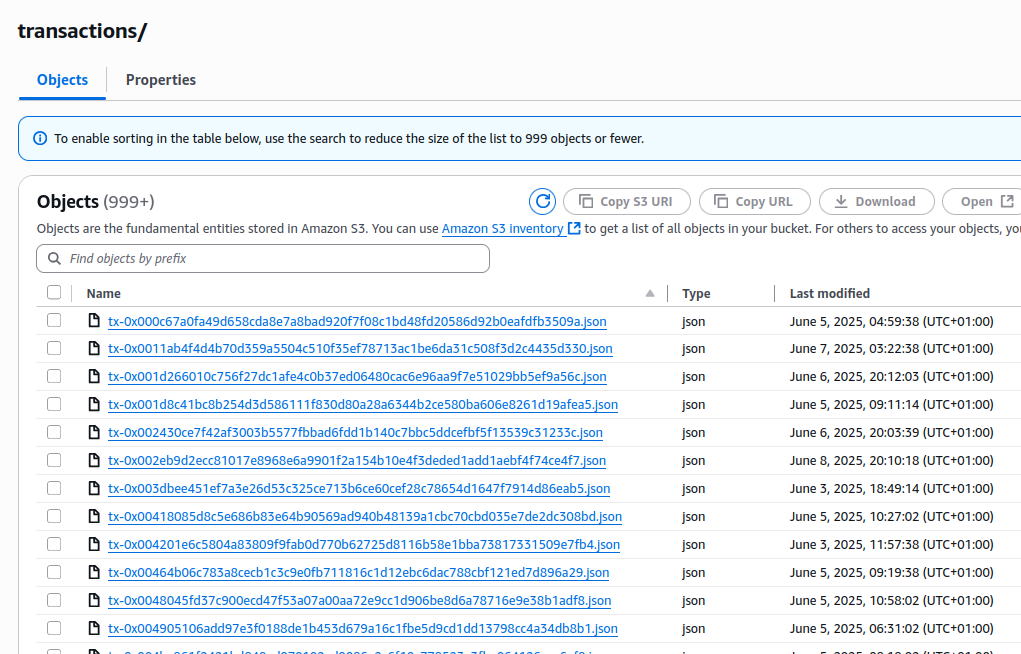
\includegraphics[scale=0.4]{AWS/events_s3_tx}
   \captionof{figure}{Almacenamiento de mensajes JSON en AWS S3.}
   \label{fig:events_s3_tx}
\end{center}


\begin{center}
   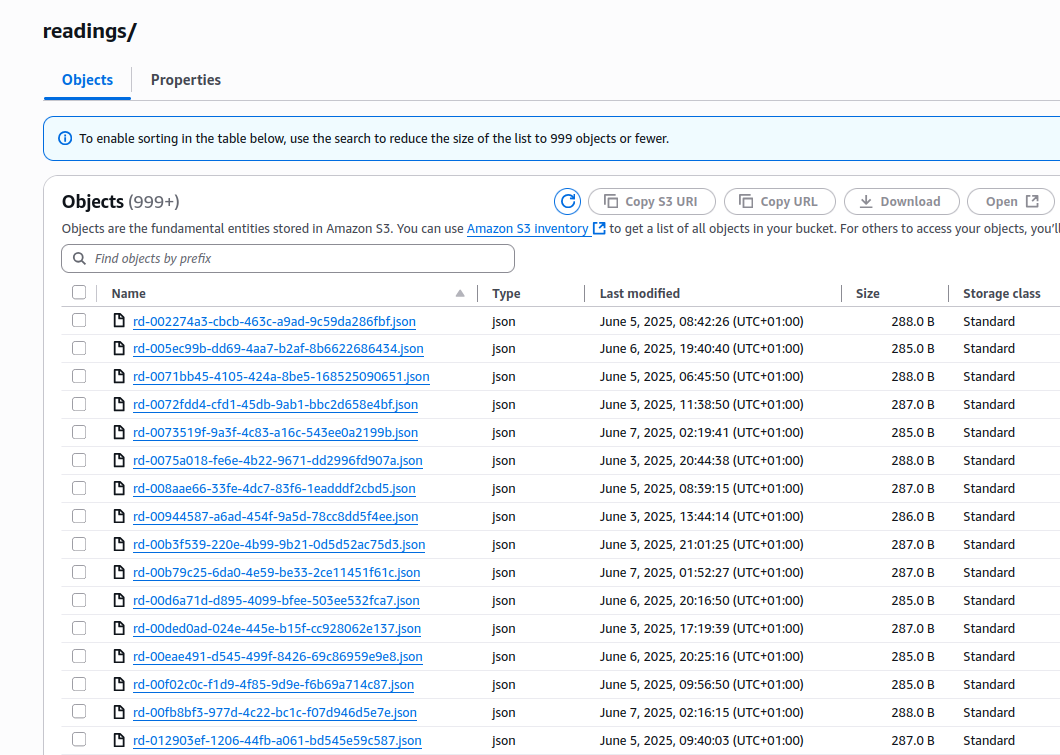
\includegraphics[scale=0.4]{AWS/events_s3_readings}
   \captionof{figure}{Almacenamiento de mensajes JSON en AWS S3.}
   \label{fig:events_s3_readings}
\end{center}


\begin{center}
   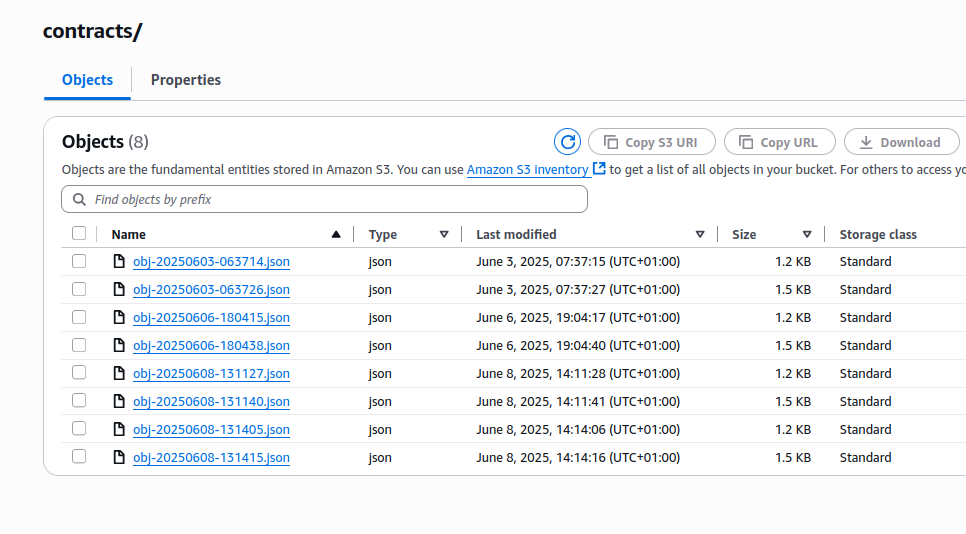
\includegraphics[scale=0.4]{AWS/events_s3_contracts}
   \captionof{figure}{Almacenamiento de mensajes JSON en AWS S3.}
   \label{fig:events_s3_contracts}
\end{center}


\subsection{Verificación del acceso a datos desde AWS Athena}



\begin{center}
   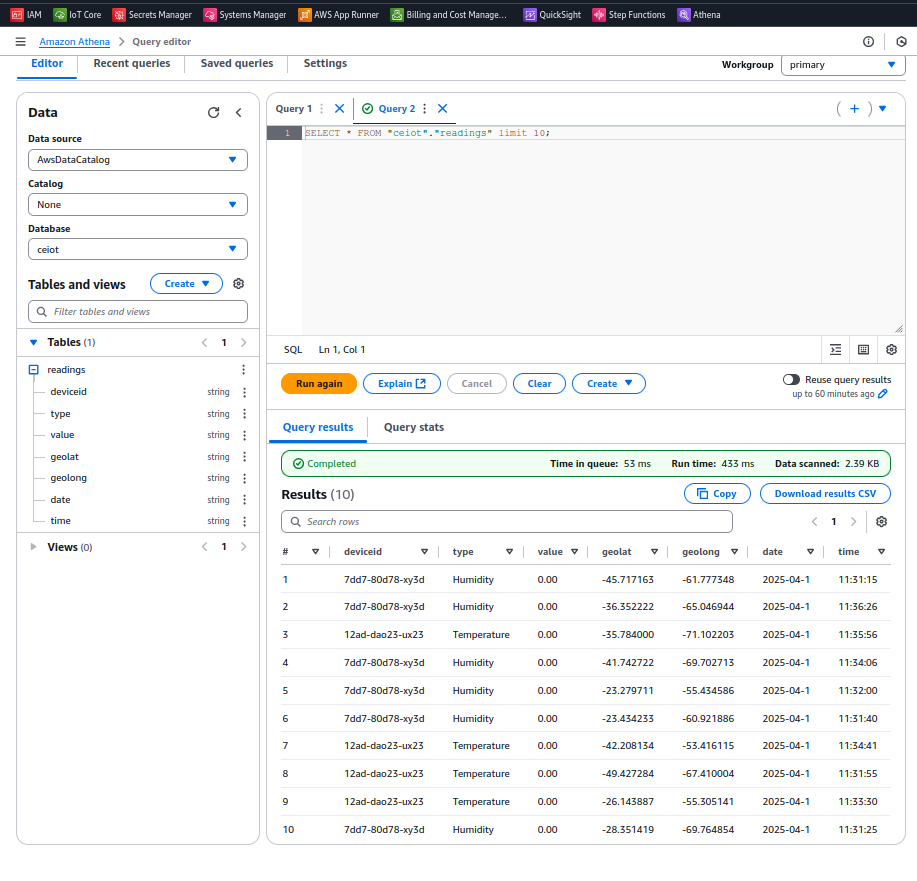
\includegraphics[scale=0.4]{AWS/aws_athena_config}
   \captionof{figure}{Consulta de datos SQL desde AWS Athena.}
   \label{fig:aws_athena_config}
\end{center}





\subsection{Verificación del proceso de ingesta y transformación de datos batch en Fabric}


\begin{center}
   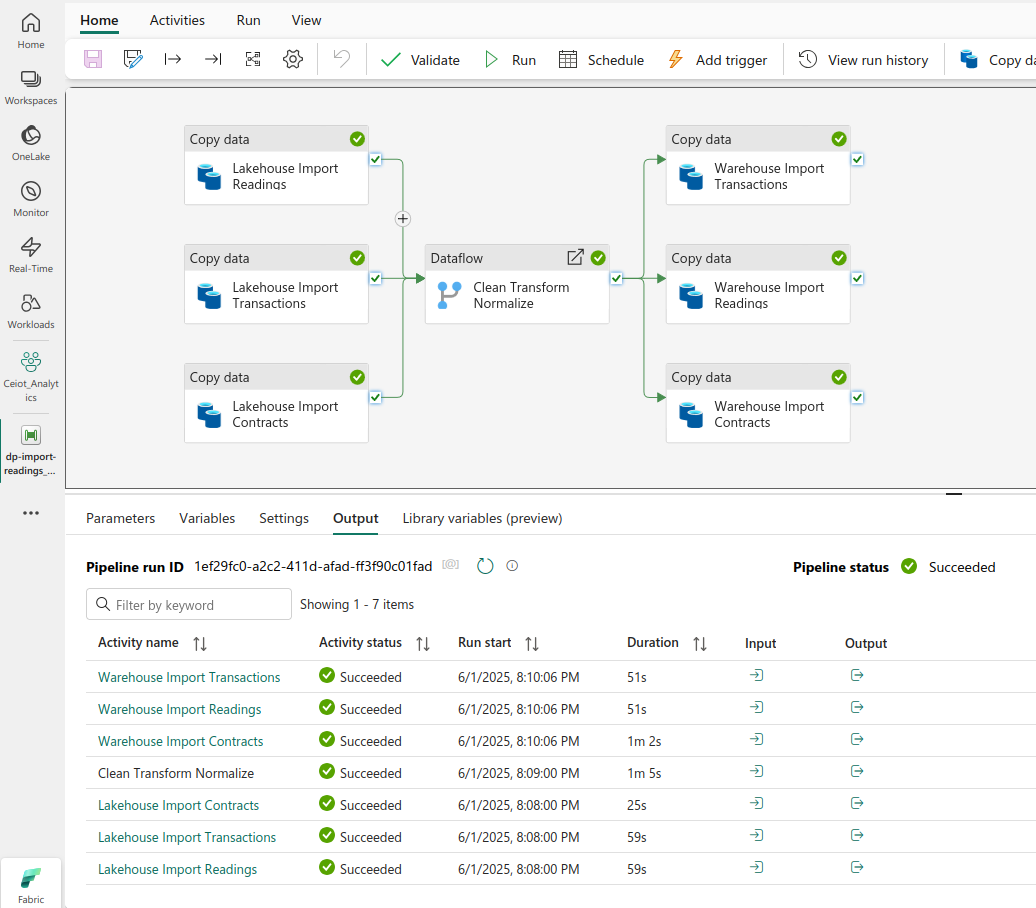
\includegraphics[scale=0.35]{Azure/datafactory_result}
   \captionof{figure}{Correcta ejecución del pipeline punta-a-punta con Azure Data Factory y Dataflows.}
   \label{fig:powerbi1}
\end{center}
 
 

\section{Validaciones funcionales del sistema}



\subsection{Validación del modelo de datos en el Semantic Model}

\subsection{Validación del reporte final generado en PowerBI}


\begin{center}
   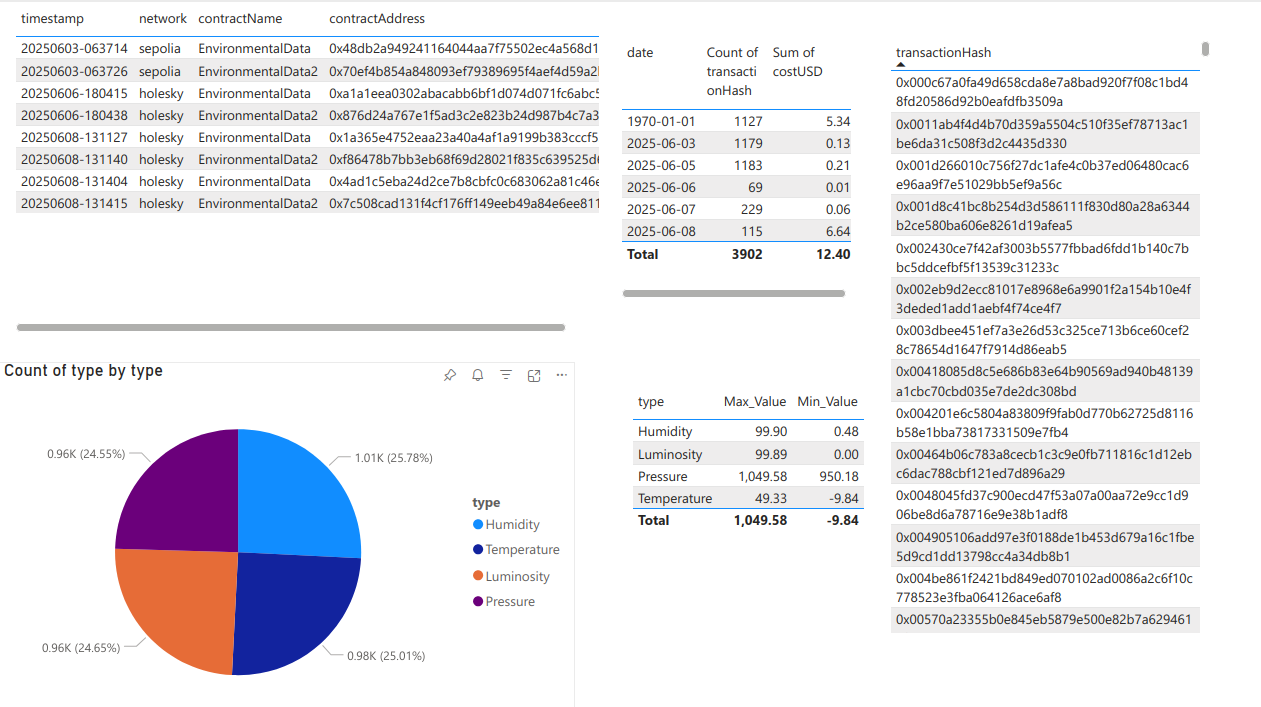
\includegraphics[scale=0.3]{Azure/powerbi_6}
   \captionof{figure}{Dashboard PowerBI.}
   \label{fig:powerbi1}
\end{center}
 
 

\begin{center}
   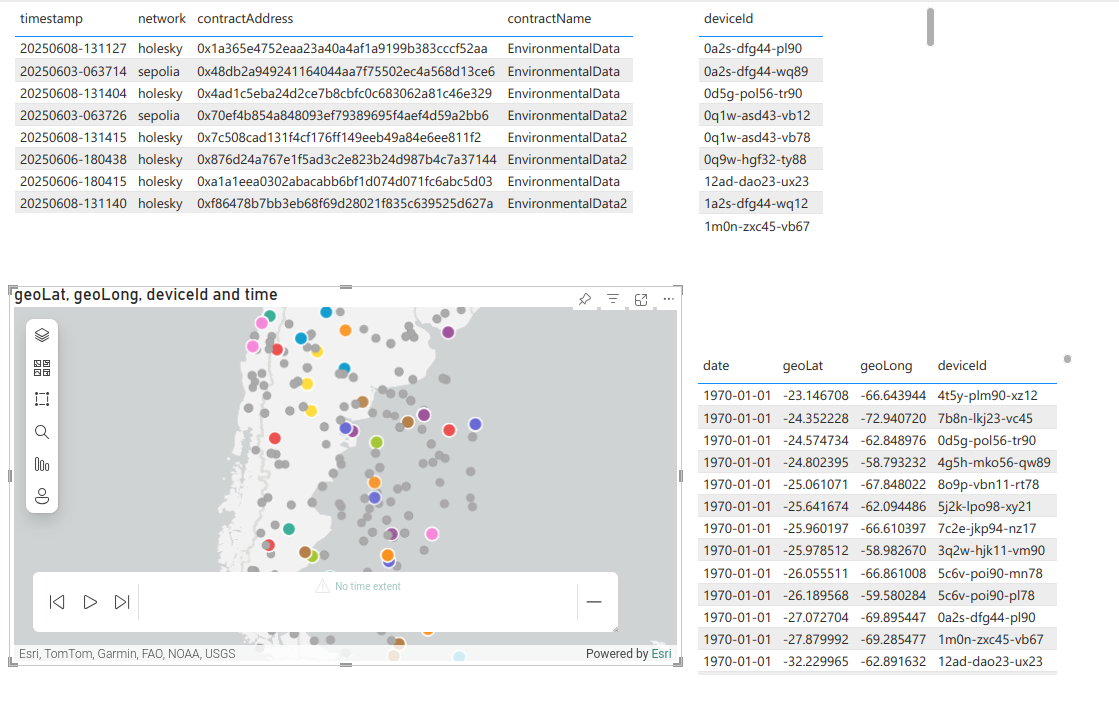
\includegraphics[scale=0.3]{Azure/powerbi_5}
   \captionof{figure}{Dashboard PowerBI.}
   \label{fig:powerbi1}
\end{center}
 


\begin{center}
   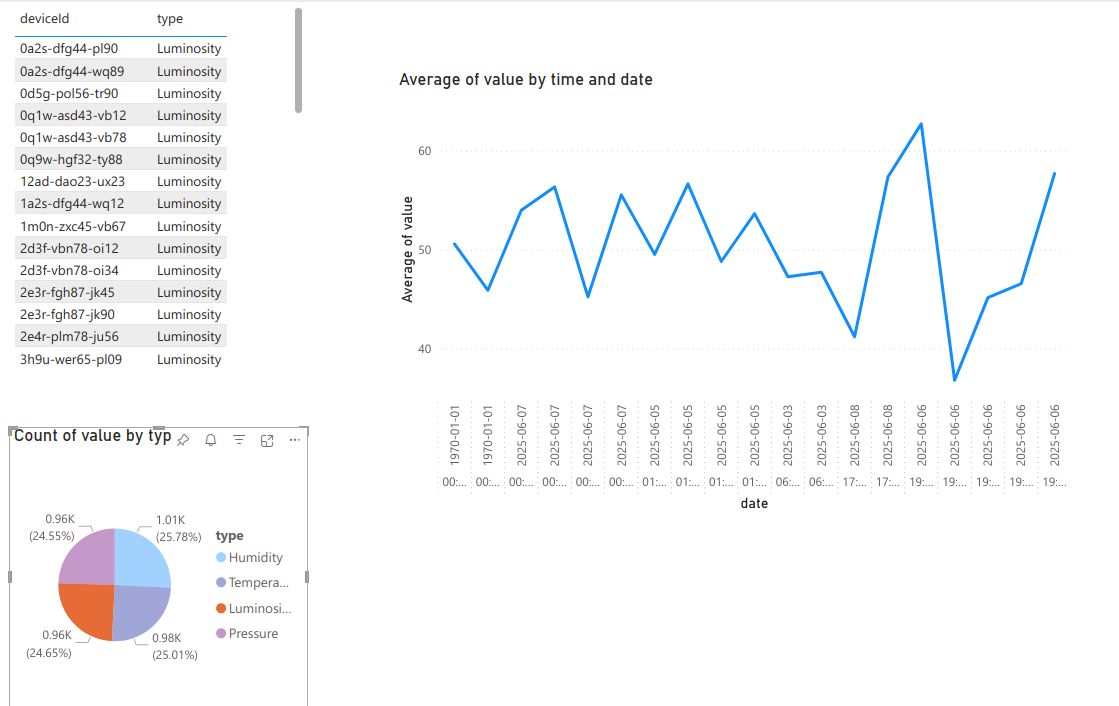
\includegraphics[scale=0.3]{Azure/powerbi_4}
   \captionof{figure}{Dashboard PowerBI.}
   \label{fig:powerbi1}
\end{center}
 
 

\begin{center}
   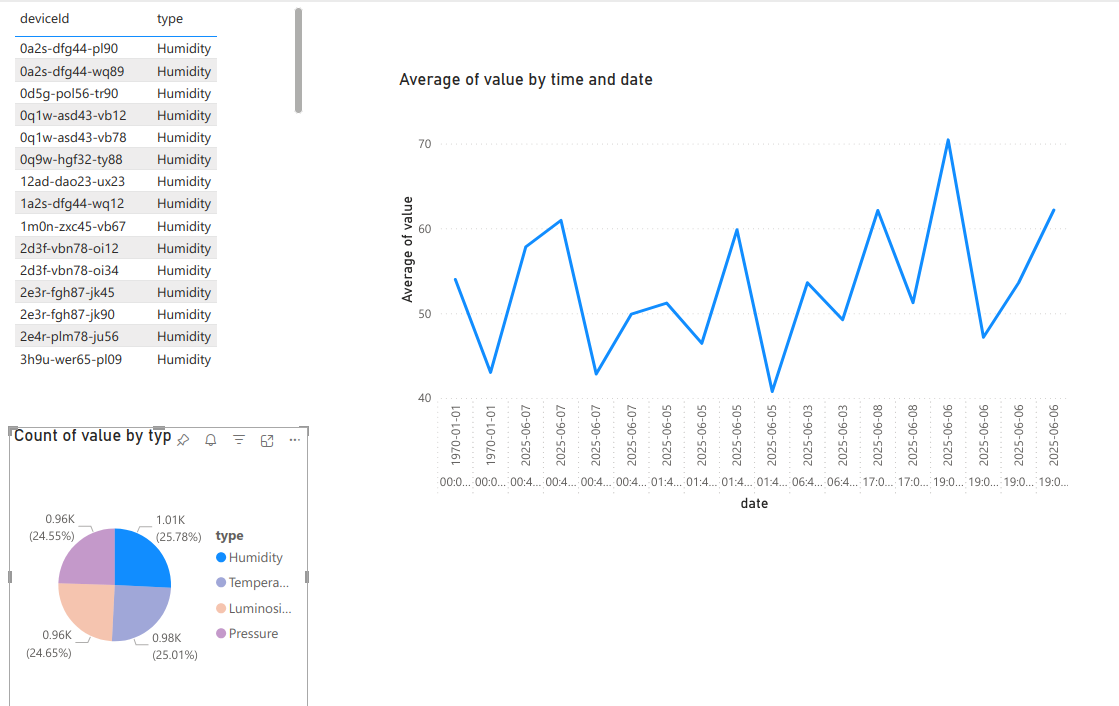
\includegraphics[scale=0.3]{Azure/powerbi_3}
   \captionof{figure}{Dashboard PowerBI.}
   \label{fig:powerbi1}
\end{center}
 
 

\begin{center}
   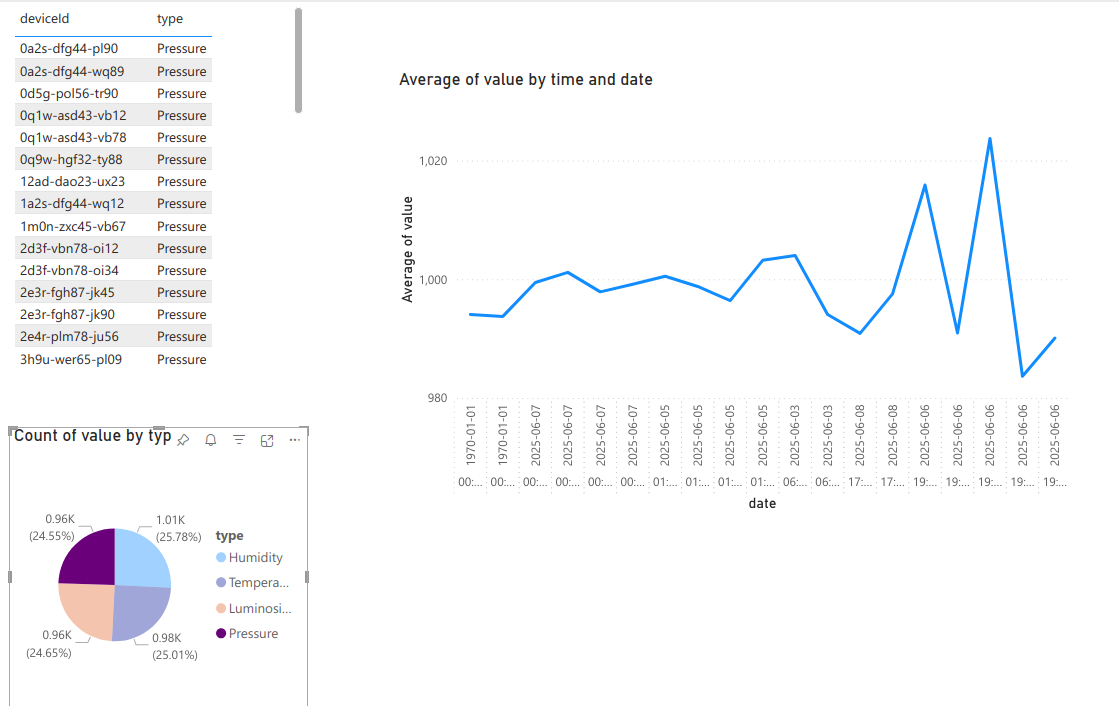
\includegraphics[scale=0.3]{Azure/powerbi_2}
   \captionof{figure}{Dashboard PowerBI.}
   \label{fig:powerbi1}
\end{center}
 
 
